% Transcrito de Documento_Visao_MotivaFit_Completo_e_Detalhado.pdf
\clearpage
\section{PROCESSO DE DESENVOLVIMENTO DE SOFTWARE}

O fluxo de trabalho unifica a estrutura de gestão do Scrum com práticas de engenharia do eXtreme Programming (XP) [4, 5]. O gerenciamento estrutura entregas em Sprints iterativas curtas. O desenvolvimento é guiado por Testes Contínuos e Pair Programming. A esteira técnica utiliza Code Review constante entre a equipe e Integração Contínua (CI) via GitHub Actions, com aplicação contínua de princípios SOLID (responsabilidade única, aberto/fechado, substituição de Liskov, segregação de interfaces e inversão de dependência) e Clean Code no desenvolvimento em Java/Spring Boot.

A equipe não adotará a Daily Scrum, pois a disponibilidade dos integrantes impossibilita a realização de encontros diários. Essa decisão representa uma adaptação do processo em relação ao Scrum descrito em [5]. O acompanhamento das atividades e a comunicação de impedimentos ocorrerão pelos canais de comunicação do grupo e nas reuniões semanais de acompanhamento.

A Figura~\ref{fig:fluxo_de_trabalho} mostra o fluxo de trabalho no nível de gestão das entregas. Os requisitos partem do Product Backlog e são selecionados durante a Sprint Planning, formando o Sprint Backlog. Durante a Sprint de uma semana, a equipe implementa os itens selecionados, aplica os testes e realiza as revisões de código e a integração contínua descritas nesta seção. Essas práticas técnicas ocorrem dentro da etapa Sprint, embora não estejam detalhadas na imagem.

A etapa Review \& Retro reúne a avaliação da entrega e a reflexão sobre o processo. A Review verifica o resultado com os interessados; a Retrospectiva orienta ajustes para o próximo ciclo. O incremento corresponde à parte concluída do produto. Os itens pendentes ou as novas necessidades retornam ao planejamento das próximas Sprints [5].

\begin{figure}[htbp]
\centering
\caption{Fluxo de trabalho do projeto}
\label{fig:fluxo_de_trabalho}
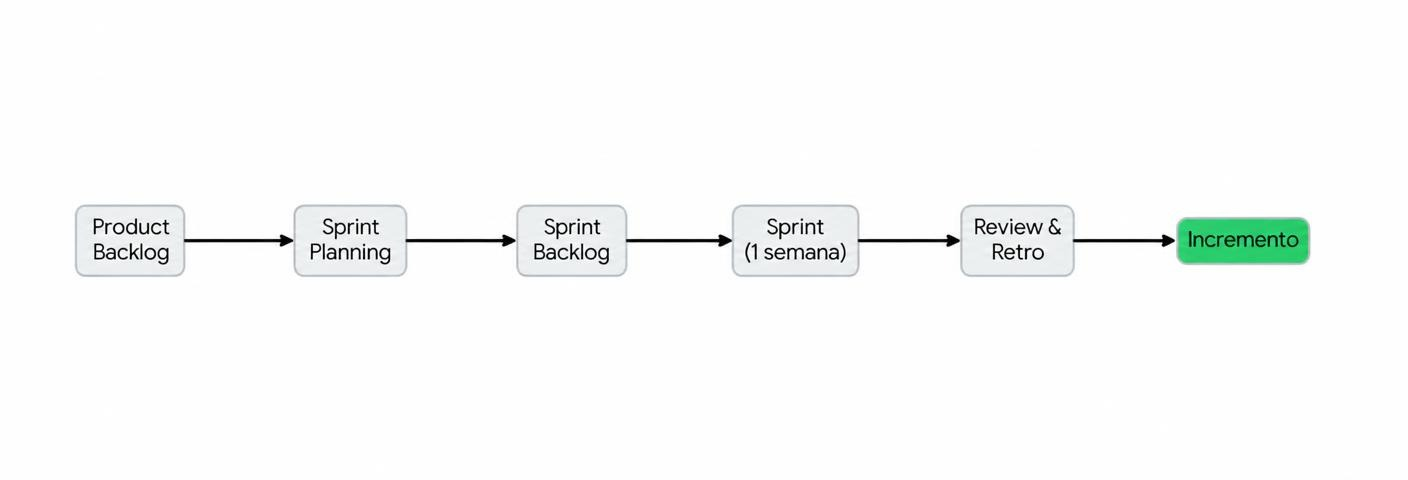
\includegraphics[width=\linewidth,keepaspectratio]{imgs/fluxo_de_trabalho.jpeg}
\par\smallskip
{\fontedez Fonte: elaborado pelos autores (2026), com base no Guia do Scrum [5].}
\end{figure}
\FloatBarrier

